%==========================================================================
% Midterm Progress Presentation
% Renewable Intermittency and Grid Reliability: A Directed Technical Change
% Model of Vietnam
% Toan T. Nguyen — Fulbright University Vietnam, Spring 2026
%==========================================================================
\documentclass[aspectratio=169,10pt]{beamer}

%--- Theme & colors -----------------------------------------------------------
\usetheme{AnnArbor}
\usecolortheme{beaver}

\definecolor{fuvblue}{RGB}{11,36,71}      % deep navy
\definecolor{fuvteal}{RGB}{13,148,136}    % teal accent
\definecolor{fuvgold}{RGB}{245,158,11}    % amber
\definecolor{fuvred}{RGB}{185,28,28}      % alert red

\setbeamercolor{palette primary}   {bg=fuvblue,  fg=white}
\setbeamercolor{palette secondary} {bg=fuvblue!85!black, fg=white}
\setbeamercolor{palette tertiary}  {bg=fuvblue!70!black, fg=white}
\setbeamercolor{palette quaternary}{bg=fuvblue,  fg=white}
\setbeamercolor{structure}         {fg=fuvblue}
\setbeamercolor{title}             {fg=white}
\setbeamercolor{frametitle}        {bg=fuvblue, fg=white}
\setbeamercolor{block title}       {bg=fuvblue!90, fg=white}
\setbeamercolor{block body}        {bg=fuvblue!6}
\setbeamercolor{block title alerted}{bg=fuvred!85, fg=white}
\setbeamercolor{block body alerted} {bg=fuvred!7}
\setbeamercolor{block title example}{bg=fuvteal!85, fg=white}
\setbeamercolor{block body example} {bg=fuvteal!7}
\setbeamercolor{item projected}{bg=fuvteal, fg=white}
\setbeamercolor{itemize item}{fg=fuvteal}
\setbeamercolor{itemize subitem}{fg=fuvblue!60}
\setbeamercolor{enumerate item}{fg=fuvteal}

\setbeamertemplate{navigation symbols}{}     % clean — no nav symbols
\setbeamerfont{frametitle}{size=\large, series=\bfseries}
\setbeamerfont{title}{size=\Large, series=\bfseries}

%--- Packages -----------------------------------------------------------------
\usepackage{amsmath,amssymb,amsthm}
\usepackage{booktabs,multirow}
\usepackage{graphicx}
\usepackage{tikz}
\usetikzlibrary{arrows.meta,positioning,shapes.geometric,fit,backgrounds}
\usepackage{pgfplots}
\pgfplotsset{compat=1.18}
\usepackage{xcolor}
\usepackage{tcolorbox}
\tcbuselibrary{skins,breakable}
\usepackage{array}
\usepackage{microtype}

%--- Custom environments ------------------------------------------------------
\newcommand{\fuvhl}[1]{\textcolor{fuvteal}{\textbf{#1}}}
\newcommand{\fuvem}[1]{\textcolor{fuvgold}{\textbf{#1}}}
\newcommand{\fuvwarn}[1]{\textcolor{fuvred}{\textbf{#1}}}
\newcommand{\hh}{\hat}

\newtcolorbox{keybox}[1][]{
  colback=fuvteal!8, colframe=fuvteal!70, fonttitle=\bfseries\small,
  boxrule=0.6pt, arc=2pt, left=4pt, right=4pt, top=3pt, bottom=3pt, #1
}
\newtcolorbox{alertbox}[1][]{
  colback=fuvred!7, colframe=fuvred!70, fonttitle=\bfseries\small,
  boxrule=0.6pt, arc=2pt, left=4pt, right=4pt, top=3pt, bottom=3pt, #1
}
\newtcolorbox{goldbox}[1][]{
  colback=fuvgold!10, colframe=fuvgold!80, fonttitle=\bfseries\small,
  boxrule=0.6pt, arc=2pt, left=4pt, right=4pt, top=3pt, bottom=3pt, #1
}

%--- Footline with slide counter ----------------------------------------------
\setbeamertemplate{footline}{%
  \leavevmode%
  \hbox{%
    \begin{beamercolorbox}[wd=.33\paperwidth,ht=2.25ex,dp=1ex,left,leftskip=4pt]{palette primary}%
      \usebeamerfont{author in head/foot}\insertshortauthor
    \end{beamercolorbox}%
    \begin{beamercolorbox}[wd=.34\paperwidth,ht=2.25ex,dp=1ex,center]{palette primary}%
      \usebeamerfont{title in head/foot}\insertshorttitle
    \end{beamercolorbox}%
    \begin{beamercolorbox}[wd=.33\paperwidth,ht=2.25ex,dp=1ex,right,rightskip=4pt]{palette primary}%
      \usebeamerfont{date in head/foot}
      \insertframenumber{} / \inserttotalframenumber
    \end{beamercolorbox}%
  }%
}

%--- Title information --------------------------------------------------------
\title[Vietnam DSGE --- Midterm Update]{%
  \textbf{Renewable Intermittency and Grid Reliability}\\[4pt]
  \normalsize An Endogeneous Learning Model for Vietnam\\[2pt]
  \small\textit{Midterm Progress Report}%
}
\author[Toan T.\ Nguyen]{%
  \textbf{Toan T.\ Nguyen (Justin)}\\[2pt]
  {\small Advisor: Dr.\ Xavier Martin G.\ Bautista}%
}
\institute[Fulbright University Vietnam]{%
  Fulbright University Vietnam
}
\date{Spring 2026}

%==========================================================================
\begin{document}
%==========================================================================

%--- SLIDE 1: Title --------------------------------------------------------
\begin{frame}[plain]
  \titlepage
\end{frame}

%--- SLIDE 2: Outline -------------------------------------------------------
\begin{frame}{Presentation Outline}
  \tableofcontents[hideallsubsections]
\end{frame}

%==========================================================================
\section{Motivation \& Research Questions}
%==========================================================================

%--- SLIDE 3: The Energy Trilemma ------------------------------------------
\begin{frame}{Vietnam's Energy Trilemma}
  \begin{columns}[T]
    \begin{column}{0.47\textwidth}
      Vietnam's growth model confronts three simultaneously binding constraints:
      \medskip
      \begin{itemize}
        \item \fuvhl{Energy security:} rapidly rising industrial demand
        \item \fuvhl{Sustainability:} Paris Agreement + Net Zero pledges
        \item \fuvhl{Affordability:} administratively regulated retail tariffs (EVN)
      \end{itemize}
      \medskip
      \begin{keybox}[title=PDP8 at a Glance]
        \small
        \begin{tabular}{@{}lll@{}}
          & \textbf{2024 actual} & \textbf{2030 target}\\
          \midrule
          Solar + Wind & 22.8 GW & 73.5 GW\\
          Battery BESS & 0.25 GW & 14.0 GW\\
          Grid invest.\ & \$3.2 B/yr & \$3.6 B/yr\\
        \end{tabular}
      \end{keybox}
    \end{column}
    \begin{column}{0.50\textwidth}
      \begin{alertbox}[title=The Core Structural Friction]
        \small Renewable generation is \textit{non-dispatchable}: supply clears in real time with demand. As VRE penetration rises without adequate storage, the \textbf{reliability penalty}---endogenous reduction in capital utilization from grid instability---acts like a persistent negative TFP shock.
      \end{alertbox}
      \vspace{0.3em}
      \begin{goldbox}[title=Empirical Trigger]
        \small Solar capacity doubled in 18 months (2020–21) under FiT incentives, while battery storage remained near zero. Vietnam already experiences curtailment $>$10\% in southern provinces.
      \end{goldbox}
    \end{column}
  \end{columns}
\end{frame}

%--- SLIDE 4: Literature Gap -----------------------------------------------
\begin{frame}{Literature Gap: What Existing Models Miss}
  \begin{columns}[T]
    \begin{column}{0.48\textwidth}
      \textbf{\textcolor{fuvblue}{What the literature covers:}}
      \begin{itemize}\small
        \item \textit{E-DSGE models} (Heutel 2012; Airaudo et al.\ 2025): carbon taxes, ``greenflation''
        \item \textit{Directed Technical Change} (Acemoglu et al.\ 2012): R\&D-race between sectors
        \item \textit{Techno-economic} (Zakeri \& Syri 2015; Schreiner 2020): storage costs, grid investment
        \item \textit{Open economy} (Schmitt-Grohé 2003): debt-elastic interest rates
      \end{itemize}
    \end{column}
    \begin{column}{0.48\textwidth}
      \textbf{\textcolor{fuvred}{Critical blind spots:}}
      \begin{itemize}\small
        \item No model \textit{endogenizes grid reliability} as a capital utilization constraint
        \item DTC literature ignores \textit{deployment-driven learning} in storage
        \item Public--private investment \textit{asymmetry} (``agility gap'') is not formalized
        \item Open-economy E-DSGE ignores \textit{battery import price} as a terms-of-trade shock
      \end{itemize}
      \vspace{0.3em}
      \begin{keybox}
        \small \textbf{This capstone} bridges all four gaps jointly---in a single DSGE calibrated to Vietnam.
      \end{keybox}
    \end{column}
  \end{columns}
\end{frame}

%--- SLIDE 5: Research Questions -------------------------------------------
\begin{frame}{Research Questions \& Contributions}
  \begin{block}{Four Research Questions}
    \begin{enumerate}\small
      \item How does VRE intermittency propagate through capital utilization into macroeconomic output losses?
      \item What is the structural timing mismatch between private battery and public grid investment---the \textbf{Agility Gap}?
      \item How does endogenous learning-by-doing in storage depend on regulatory price signal transmission ($\chi$)?
      \item What are the welfare costs of intermittency and how do policy instruments rank in closing the gap?
    \end{enumerate}
  \end{block}
  \medskip
  \begin{columns}[T]
    \begin{column}{0.31\textwidth}
      \begin{keybox}[title=Contribution 1]
        \small Endogenous reliability function: $u_t = f(\text{flexibility}/\text{VRE vol})$
      \end{keybox}
    \end{column}
    \begin{column}{0.31\textwidth}
      \begin{keybox}[title=Contribution 2]
        \small Reliability-gap learning: $\Delta A_{bat}$ responds to scarcity signal $\chi$
      \end{keybox}
    \end{column}
    \begin{column}{0.31\textwidth}
      \begin{keybox}[title=Contribution 3]
        \small CES agility gap: private batteries (agile) vs.\ public grid (sluggish)
      \end{keybox}
    \end{column}
  \end{columns}
\end{frame}

%==========================================================================
\section{Model Environment}
%==========================================================================

%--- SLIDE 6: Overview diagram ----------------------------------------------
\begin{frame}{Model Architecture: Small Open Economy DSGE}
  \begin{center}
    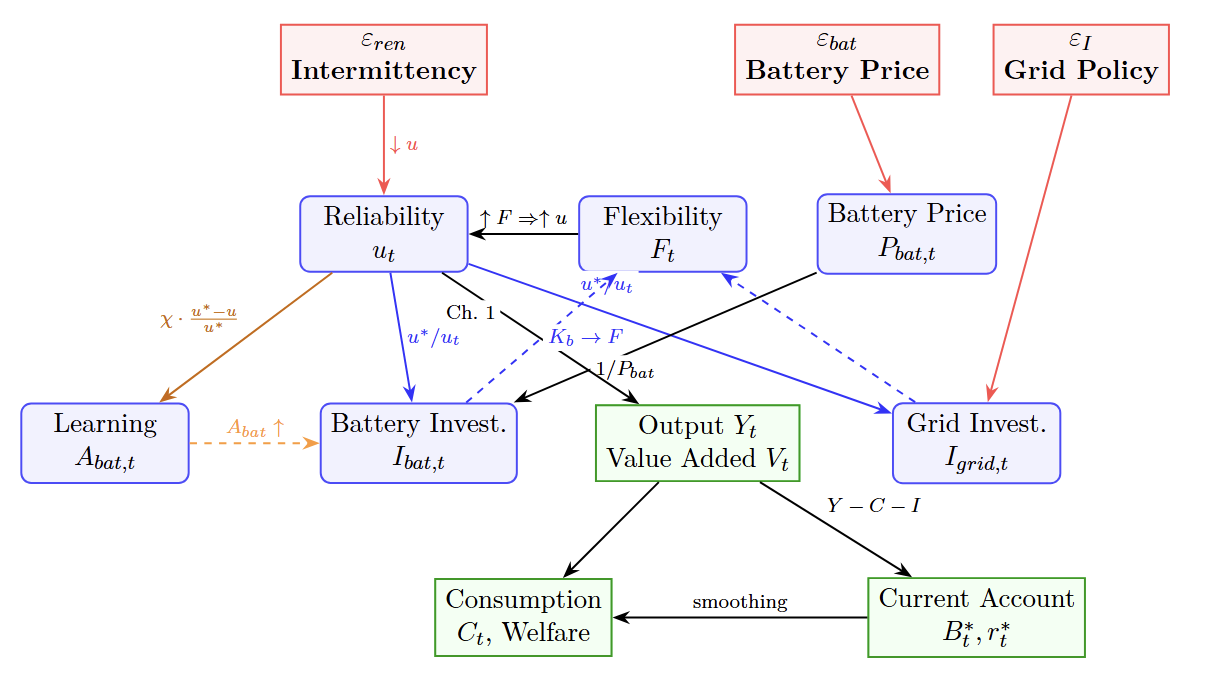
\includegraphics[width=0.82\linewidth,height=0.80\textheight,keepaspectratio]{overview_diagram.png}
  \end{center}
\end{frame}

%--- SLIDE 7: Households ---------------------------------------------------
\begin{frame}{Households}
  \begin{columns}[T]
    \begin{column}{0.47\textwidth}
      \begin{block}{Objective}
        \begin{itemize}\small
          \item Representative household maximizes discounted utility over consumption $C_t$ and labor $L_t$
          \item Standard log utility in consumption; disutility of labor
          \item Discount factor $\beta = 0.990$ (4\% annualized real return)
        \end{itemize}
      \end{block}
      \vspace{0.4em}
      \begin{block}{Budget Constraint}
        \begin{itemize}\small
          \item Income: wages $w_t L_t$, capital rental $R_t K_{p,t}$, foreign bond returns
          \item Expenditure: consumption, productive investment, \fuvhl{battery purchases} $P_{bat,t}I_{bat,t}$, taxes, foreign bonds
        \end{itemize}
      \end{block}
    \end{column}
    \begin{column}{0.47\textwidth}
      \begin{block}{Optimality Conditions}
        \begin{itemize}\small
          \item \textbf{Capital Euler:} equates marginal cost of saving today to discounted return on capital tomorrow
          \item \textbf{Bond Euler:} links domestic consumption growth to world interest rate $r^*_t$
          \item \textbf{Labor supply:} wages equal marginal disutility of work
        \end{itemize}
      \end{block}
      \vspace{0.4em}
      \begin{keybox}
        \small \textbf{Key modeling choice:} Capital utilization $u_t$ is \textit{not} a household decision. It is an exogenous physical constraint set by grid reliability---not a margin households can optimize over.
      \end{keybox}
    \end{column}
  \end{columns}
\end{frame}

%--- SLIDE 8: Production & Reliability ------------------------------------
\begin{frame}{Production \& The Two Novel Equations}
  \begin{itemize}\small
    \item Output is a CES aggregate of value-added $V_t$ and energy $\bar{E}$ (substitutability $\sigma_E = 0.6$)
    \item Value-added is Cobb-Douglas with capital share $\alpha = 0.35$ --- but effective capital is \fuvhl{$u_t K_{p,t}$}, so grid reliability directly reduces productive capacity
  \end{itemize}
  \vspace{0.3em}
  \begin{columns}[T]
    \begin{column}{0.47\textwidth}
      \begin{alertbox}[title=\textbf{Contribution 1} --- Reliability Constraint]
        \[
          u_t = 1 - \exp\!\left(-\psi\,\frac{F_t}{\phi_{int}\cdot\mathrm{Vol}_{ren,t}}\right)
        \]
        \small Utilization rises as the \textit{flexibility stock} $F_t$ grows relative to VRE volatility. The exponential form captures nonlinear reliability costs. When $F_t \uparrow$ or volatility $\downarrow$, $u_t \to 1$.
      \end{alertbox}
    \end{column}
    \begin{column}{0.47\textwidth}
      \begin{keybox}[title=\textbf{Contribution 2} --- CES Flexibility Bundle]
        \[
          F_t = \!\left[\mu(A_{bat,t}K_{b,t})^{\frac{\rho_f-1}{\rho_f}}
          +(1{-}\mu)K_{g,t}^{\frac{\rho_f-1}{\rho_f}}\right]^{\frac{\rho_f}{\rho_f-1}}
        \]
        \small Batteries and grid are \textit{complements} ($\rho_f=0.4 < 1$): neither can substitute for the other when the opposing asset is scarce. $A_{bat,t}$ captures endogenous learning.
      \end{keybox}
    \end{column}
  \end{columns}
\end{frame}

%--- SLIDE 9: Battery Investment & Learning --------------------------------
\begin{frame}{Battery Investment \& Endogenous Learning}
  \begin{columns}[T]
    \begin{column}{0.47\textwidth}
      \begin{block}{Battery Investment (Private, Agile)}
        \begin{itemize}\small
          \item Investment responds \textit{contemporaneously} to the reliability gap $(u^* - u_t)$: the larger the shortfall, the more private capital is deployed
          \item Dampened by the world battery price $P_{bat,t}$ --- Vietnam is a price-taker on global lithium markets
          \item Capital accumulates each period net of 12\% annual depreciation (Li-ion lifecycle)
        \end{itemize}
      \end{block}
    \end{column}
    \begin{column}{0.47\textwidth}
      \begin{alertbox}[title=\textbf{Contribution 3} --- Endogenous Learning]
        \begin{itemize}\small
          \item Battery productivity $A_{bat,t}$ improves when the reliability gap is large: scarcity drives learning-by-doing
          \item Learning speed $\eta_{bat} = 0.10$ anchored to the 18--22\% Li-ion experience curve
          \item \fuvhl{$\chi \in [0,1]$}: regulatory transmission parameter — how well market prices signal scarcity
          \item \fuvwarn{Vietnam ($\chi = 0.3$):} regulated EVN tariffs suppress the scarcity signal, slowing battery cost reduction
        \end{itemize}
      \end{alertbox}
    \end{column}
  \end{columns}
  \vspace{0.2em}
  \begin{goldbox}
    \small \textbf{Agility Gap:} Private batteries respond to reliability shortfalls \textit{immediately}; public grid investment lags 5--7 years due to permitting and construction. This asymmetry generates the mid-transition reliability valley.
  \end{goldbox}
\end{frame}

%==========================================================================
\section{Model Mechanics \& Log-Linearization}
%==========================================================================



%--- SLIDE 17: Transmission channels --------------------------------------
\begin{frame}{Three Transmission Channels}
  \begin{block}{Channel 1 --- The Reliability Wedge (Output Loss)}
    \small An intermittency shock raises VRE volatility $\Rightarrow$ reliability $u_t$ falls $\Rightarrow$ effective capital $u_t K_{p,t}$ shrinks $\Rightarrow$ output $Y_t$ falls. Acts like a persistent, supply-side negative TFP shock, amplified by energy--capital complementarity.
  \end{block}
  \vspace{0.3em}
  \begin{block}{Channel 2 --- The Agility Gap (Asymmetric Investment)}
    \small When $u_t < u^*$: private batteries invest \textit{immediately} (agile); public grid investment responds but faces 5--7 year construction lags (sluggish). The timing mismatch generates a predictable mid-transition reliability valley.
  \end{block}
  \vspace{0.3em}
  \begin{block}{Channel 3 --- Reliability-Gap Learning (Innovation)}
    \small A reliability shortfall triggers endogenous battery cost reduction via learning-by-doing. The speed of learning depends on $\chi$: regulated tariffs suppress scarcity signals, slowing the innovation response and deepening the ``valley of death'' for storage technology.
  \end{block}
\end{frame}

%==========================================================================
\section{Preliminary Results}
%==========================================================================

%==========================================================================
\section{Work in Progress}
%==========================================================================

%--- SLIDE 24: Work in progress --------------------------------------------
\begin{frame}{Work in Progress}
  \begin{columns}[T]
    \begin{column}{0.47\textwidth}
      \begin{block}{\textcolor{fuvteal}{Completed} \checkmark}
        \begin{itemize}\small
          \item Full model derivation (16-equation equilibrium)
          \item Analytical steady-state characterization \& solver
          \item Dynare implementation \& Blanchard-Kahn verification
          \item Impulse response functions (3 shocks)
          \item Deterministic transition simulation (Reliability Valley)
          \item Log-linearization \& transmission channel analysis
        \end{itemize}
      \end{block}
    \end{column}
    \begin{column}{0.47\textwidth}
      \begin{alertbox}[title=\textcolor{fuvred}{In Progress / Remaining}]
        \begin{itemize}\scriptsize
          \item Full calibration (structural + reliability + LBD blocks)
          \item \textbf{Welfare analysis:} consumption-equivalent variation $\Lambda(\chi)$
          \item \textbf{Counterfactual experiments:}
            battery subsidy ($P_{bat}=0.8$); accelerated grid ($\phi_{grid}=3.0$); signal suppression ($\chi=0.3$)
          \item \textbf{``Perfect Storm'' scenario:} joint $\varepsilon_{ren}+\varepsilon_{bat}$ simulation
          \item \textbf{Sensitivity analysis:} $\psi$, $\mu$, $\beta$, $\phi_{grid}$
          \item \textbf{Formal propositions:} prove $\Lambda(\chi)$ monotonicity and CES supermodularity
          \item \textbf{Policy section:} map $\chi\to$ concrete EVN reform agenda
          \item \textbf{LaTeX manuscript:} finalize bibliography \& appendix proofs
        \end{itemize}
      \end{alertbox}
    \end{column}
  \end{columns}
\end{frame}

%--- SLIDE 26: Summary of Contributions ------------------------------------
\begin{frame}{Summary: Three Contributions to the Literature}
  \begin{enumerate}
    \item \textbf{Endogenous Grid Reliability as a Macro Friction}\\[2pt]
    {\small Capital utilization $u_t = 1-\exp(-\psi F_t/\phi_{int}\mathrm{Vol}_{ren,t})$ is determined endogenously by the stock of flexibility assets relative to VRE volatility. This transforms an engineering concept into a macroeconomic wedge in the aggregate production function---a channel absent from all extant E-DSGE models.}
    \medskip

    \item \textbf{Reliability-Gap-Induced Learning-by-Doing}\\[2pt]
    {\small Battery technology evolves endogenously: $\Delta A_{bat} = \eta_{bat}\cdot\chi\cdot(u^*-u)/u^*$. Unlike DTC models that require explicit R\&D sectors, innovation here responds to \textit{deployment-driven scarcity}. The regulatory parameter $\chi$ maps directly to observable policy instruments. \textbf{Policy Rec:} Vietnam must establish dynamic capacity markets (raising $\chi$) to unlock storage cost reductions.}
    \medskip

    \item \textbf{Identification of the Structural Agility Gap}\\[2pt]
    {\small Private batteries (agile, price-driven) and public grid capital (sluggish, rule-based) are formally distinguished as \textit{complementary} inputs in a CES flexibility bundle ($\rho_f=0.4$). This generates a predictable mid-transition reliability valley---a quantitative prediction unavailable in models that treat flexibility as homogeneous.}
  \end{enumerate}
\end{frame}

%--- SLIDE 27: Key References ---------------------------------------------
\begin{frame}{Key References}
  \begin{columns}[T]
    \begin{column}{0.48\textwidth}
      \textbf{\textcolor{fuvblue}{Macro \& DSGE Foundations}}
      \begin{itemize}\scriptsize
        \item Heutel, G. (2012). How should environmental policy respond to business cycles? \textit{AEJ: Economic Policy}, 4(2), 39--66.
        \item Schmitt-Grohé, S.\ \& Uribe, M.\ (2003). Closing small open economy models. \textit{Journal of International Economics}, 61(1), 163--185.
        \item Acemoglu, D.\ et al.\ (2012). The environment and directed technical change. \textit{AER}, 102(1), 131--166.
        \item Adjemian, S.\ et al.\ (2024). \textit{Dynare: Reference Manual, Version~6}. CEPREMAP.
      \end{itemize}
      \vspace{0.4em}
      \textbf{\textcolor{fuvblue}{Energy \& Storage Economics}}
      \begin{itemize}\scriptsize
        \item Zakeri, B.\ \& Syri, S.\ (2015). Electrical energy storage systems. \textit{Renewable \& Sustainable Energy Reviews}, 42, 569--596.
        \item Hart, E.K.\ (2019). Quantifying the challenge of reaching a 100\% renewable energy power system. \textit{Joule}, 3(10), 2379--2384.
        \item Hirth, L.\ (2013). The market value of variable renewables. \textit{Energy Economics}, 38, 218--236.
      \end{itemize}
    \end{column}
    \begin{column}{0.48\textwidth}
      \textbf{\textcolor{fuvblue}{Learning \& Experience Curves}}
      \begin{itemize}\scriptsize
        \item Kittner, N.\ et al.\ (2017). Energy storage deployment and innovation for the clean energy transition. \textit{Nature Energy}, 2, 17125.
        \item Way, R.\ et al.\ (2022). Empirically grounded technology forecasts and the energy transition. \textit{Joule}, 6(9), 2057--2082.
      \end{itemize}
      \vspace{0.4em}
      \textbf{\textcolor{fuvblue}{Vietnam-Specific Data}}
      \begin{itemize}\scriptsize
        \item GSO (2024). \textit{Statistical Yearbook of Vietnam 2023}. General Statistics Office.
        \item IEA (2023). \textit{Vietnam Energy Outlook 2023}. International Energy Agency.
        \item EVN (2023). \textit{Annual Report on Grid Reliability}. Electricity of Vietnam.
        \item BNEF (2023). \textit{Li-ion Battery Price Survey}. BloombergNEF.
        \item Vietnam Ministry of Industry \& Trade (2023). \textit{Power Development Plan 8 (PDP8)}.
      \end{itemize}
    \end{column}
  \end{columns}
\end{frame}

%--- SLIDE 28: Final slide -------------------------------------------------
\begin{frame}{Thank You}
  \begin{center}
    \vspace{0.5em}
    {\Large \textbf{Renewable Intermittency and Grid Reliability:}}\\[4pt]
    {\large An Endogeneous Learning Model of Vietnam}\\[8pt]
    {\normalsize \textit{Midterm Progress Report}}
    \vspace{1em}

    \begin{keybox}[title=Contact]
      \centering
      \textbf{Toan T.\ Nguyen (Justin)}\\
      Fulbright University Vietnam\\[4pt]
      \texttt{toan.nguyen.220107@student.fulbright.edu.vn}\\[4pt]
      Advisor: Dr.\ Xavier Martin G.\ Bautista
    \end{keybox}
    \vspace{1em}

    {\small \textbf{Keywords:} Environmental DSGE $\cdot$ Endogenous Learning $\cdot$ Investment Inertia\\
    Renewable Intermittency $\cdot$ Energy Storage $\cdot$ Vietnam PDP8}
    \vspace{0.8em}

    {\footnotesize \textcolor{fuvblue!60}{Code repository: \texttt{vietnam\_dsge.mod} + \texttt{run\_dynare.m} (MATLAB/Dynare 6)}}
  \end{center}
\end{frame}

%==========================================================================
%  APPENDIX
%==========================================================================
\appendix

%--- APPENDIX: Household equations ----------------------------------------
\begin{frame}{Appendix: Household Equations}
  \begin{columns}[T]
    \begin{column}{0.47\textwidth}
      \begin{block}{Lifetime Utility \& Budget Constraint}
        \[
          \max \;\mathbb{E}_0 \sum_{t=0}^{\infty}\beta^t
          \!\left[\log C_t - \frac{L_t^{1+\sigma_L}}{1+\sigma_L}\right]
        \]
        \begin{align*}
          &C_t + I_{p,t} + P_{bat,t}I_{bat,t} + B^*_t + T_t\\
          &\quad= w_t L_t + R_t K_{p,t} + (1+r^*_{t-1})B^*_{t-1}
        \end{align*}
      \end{block}
    \end{column}
    \begin{column}{0.47\textwidth}
      \begin{block}{Optimality Conditions}
        \textit{Capital Euler:}
        \[
          \frac{1}{C_t}=\beta\,\mathbb{E}_t\!\left[\frac{\alpha Y_{t+1}/K_{p,t+1}+1-\delta_p}{C_{t+1}}\right]
        \]
        \textit{Labor Supply:}
        \[
          (1-\alpha)V_t = \varphi\,C_t\,L_t^{1+\sigma_L}
        \]
      \end{block}
    \end{column}
  \end{columns}
\end{frame}

%--- APPENDIX: Production equations ----------------------------------------
\begin{frame}{Appendix: Production Technology}
  \textbf{Final output} (CES, $\sigma_E = 0.6$):
  \[
    Y_t = \bigl[s_V\,V_t^{(\sigma_E-1)/\sigma_E} + (1-s_V)\bar{E}^{(\sigma_E-1)/\sigma_E}\bigr]^{\sigma_E/(\sigma_E-1)}
  \]
  \textbf{Value-added} (Cobb-Douglas with endogenous utilization):
  \[
    V_t = (u_t K_{p,t})^\alpha\,L_t^{1-\alpha}, \quad \alpha=0.35
  \]
  \textbf{Investment rules:}
  \[
    \frac{I_{bat,t}}{\bar{I}_{bat}} = \left(\frac{u^*}{u_t}\right)^{\phi_{grid}}\!\!\frac{1}{P_{bat,t}}
    \qquad
    \hat{I}_{grid,t} = -\phi_{grid}\,\hat{u}_t + \varepsilon_{I,t}
  \]
  \textbf{Learning-by-doing:}
  \[
    A_{bat,t} - A_{bat,t-1} = \eta_{bat}\cdot\chi\cdot\frac{u^*-u_t}{u^*}
  \]
\end{frame}

%--- APPENDIX: External sector equations -----------------------------------
\begin{frame}{Appendix: External Sector Equations}
  \textbf{Current account / resource constraint:}
  \[
    B^*_t = (1+r^*_{t-1})B^*_{t-1} + Y_t - C_t - I_{p,t} - P_{bat,t}I_{bat,t} - I_{grid,t}
  \]
  \textbf{Debt-elastic interest premium (Schmitt-Grohé 2003):}
  \[
    r^*_t = \bar{r} + \phi_b\!\left(e^{\bar{B}^*-B^*_t}-1\right), \quad \phi_b=0.001
  \]
  \textbf{Blanchard-Kahn eigenvalues:}
  \begin{keybox}
    \small $\lambda_1=1.033$, $\lambda_2=-2.229$, $\lambda_3=\infty$ (3 unstable) matching $C_t$, $Y_t$, $r^*_t$\\
    7 stable eigenvalues: $0,\;\approx0,\;0.90,\;0.97,\;0.98,\;0.99,\;0.99$ $\Rightarrow$ unique saddle-path \checkmark
  \end{keybox}
\end{frame}

%--- APPENDIX: Log-linearized system ----------------------------------------
\begin{frame}{Appendix: Full System of Log-Linearized Equations}
  \small
  The complete 16-equation linearized system (hat notation: $\hat{x}_t \equiv \ln X_t - \ln X_{ss}$):
  \begin{columns}[T]
    \begin{column}{0.47\textwidth}
      \begin{enumerate}\scriptsize
        \item Capital Euler: $\hat{C}_t = \mathbb{E}_t\hat{C}_{t+1} - \frac{\alpha r_{p,ss}}{1+r_{p,ss}}(\mathbb{E}_t\hat{Y}_{t+1}-\mathbb{E}_t\hat{K}_{p,t+1})$
        \item Bond Euler: $\hat{C}_t = \mathbb{E}_t\hat{C}_{t+1} - \frac{r^*_{ss}}{1+r^*_{ss}}\mathbb{E}_t\hat{r}^*_{t+1}$
        \item Labor: $\hat{V}_t = \hat{C}_t + (1+\sigma_L)\hat{L}_t$
        \item CES output: $\hat{Y}_t = s_V^{\sigma_E}\hat{V}_t$
        \item Value-added: $\hat{V}_t = \alpha(\hat{u}_t+\hat{K}_{p,t})+(1-\alpha)\hat{L}_t$
        \item Reliability: $\hat{u}_t = -\xi\hat{F}_t + \xi\hat{\mathrm{Vol}}_{ren,t}$
        \item Flexibility: $\hat{F}_t = s_b(\hat{A}_{bat,t}+\hat{K}_{b,t})+(1-s_b)\hat{K}_{g,t}$
        \item Battery invest: $\hat{I}_{bat,t} = -\phi_{grid}\hat{u}_t - \hat{P}_{bat,t}$
      \end{enumerate}
    \end{column}
    \begin{column}{0.47\textwidth}
      \begin{enumerate}\scriptsize
        \setcounter{enumi}{8}
        \item Battery capital: $\hat{K}_{b,t+1}=(1-\delta_b)\hat{K}_{b,t}+\frac{I_{bat,ss}}{K_{b,ss}}\hat{I}_{bat,t}$
        \item Learning: $\hat{A}_{bat,t}-\hat{A}_{bat,t-1}=-\eta_{bat}\cdot\chi\cdot\hat{u}_t$
        \item Grid invest: $\hat{I}_{grid,t}=-\phi_{grid}\hat{u}_t+\varepsilon_{I,t}$
        \item Grid capital: $\hat{K}_{g,t+1}=(1-\delta_g)\hat{K}_{g,t}+\frac{I_{grid,ss}}{K_{g,ss}}\hat{I}_{grid,t}$
        \item Prod.\ capital: $\hat{K}_{p,t+1}=(1-\delta_p)\hat{K}_{p,t}+\frac{I_{p,ss}}{K_{p,ss}}\hat{I}_{p,t}$
        \item Current account: [linearized $B^*_t$ equation]
        \item Interest premium: $\hat{r}^*_t = -\frac{\phi_b}{r^*_{ss}}B^*_t$
        \item Battery price AR(1): $\hat{P}_{bat,t}=\rho_{bat}\hat{P}_{bat,t-1}+\varepsilon^{bat}_t$
      \end{enumerate}
    \end{column}
  \end{columns}
\end{frame}

\begin{frame}{Appendix: Welfare Cost Formula}
  \begin{columns}[T]
    \begin{column}{0.52\textwidth}
      \begin{block}{Consumption-Equivalent Variation $\Lambda$ (Lucas 1987)}
        \scriptsize Permanent \% reduction in SS consumption leaving the household indifferent between the stochastic and deterministic economies:
        \[
          \Lambda = 1 - \exp\!\left[\frac{1-\beta}{1-\beta^{T+1}}\sum_{t=0}^{T}\beta^t
          \log\!\left(\frac{C_t^{shock}}{C_{ss}}\right)\right]
        \]
        $T=40$ quarters; $C_t^{shock}$ follows the IRF path.
      \end{block}
      \vspace{0.2em}
      \begin{block}{Proposition: $\Lambda(\chi)$ Strictly Decreasing}
        \scriptsize $\chi\uparrow$ $\Rightarrow$ faster $A_{bat}$ $\Rightarrow$ higher $F_t$, $u_t$, $Y_t$, $C_t$ $\Rightarrow$ lower $\Lambda$.\\[2pt]
        Proof: monotone comparative statics on linearized innovation equation.
      \end{block}
    \end{column}
    \begin{column}{0.44\textwidth}
      \begin{goldbox}[title=Preliminary Result]
        \small
        \begin{tabular}{@{}lcc@{}}
          \toprule
          $\chi$ & $\Lambda$ & $\Delta$ from baseline\\
          \midrule
          1.0 (baseline)   & 0.000054\% & ---\\
          0.5 (partial)    & 0.000063\% & +17\%\\
          0.0 (suppressed) & 0.000073\% & +35\%\\
          \bottomrule
        \end{tabular}
      \end{goldbox}
      \vspace{0.2em}
      \begin{alertbox}[title=Interpretation Caveat]
        \scriptsize $\Lambda$ magnitudes are small because linearization smooths the nonlinear reliability valley. \textit{Relative} rankings across $\chi$ are robust. Full nonlinear welfare costs will be computed at the final defense.
      \end{alertbox}
    \end{column}
  \end{columns}
\end{frame}

%--- SLIDE 10: Grid Investment & External Sector ---------------------------
\begin{frame}{Public Grid Investment \& External Sector}
	\begin{columns}[T]
		\begin{column}{0.47\textwidth}
			\begin{block}{Grid Investment (Government, Sluggish)}
				\begin{itemize}\small
					\item \textit{Reactive} rule: government invests more when reliability falls below target, with response strength $\phi_{grid} = 1.5$
					\item Financed by lump-sum taxes; Ricardian equivalence holds --- no crowding-out effect
					\item Implementation delay shock $\varepsilon_{I,t}$ captures budget cycles, permitting, and construction lags (5--7 years)
					\item Grid capital depreciates at 5\% annually (transmission infrastructure)
				\end{itemize}
			\end{block}
		\end{column}
		\begin{column}{0.47\textwidth}
			\begin{block}{Small Open Economy (Schmitt-Grohé 2003)}
				\begin{itemize}\small
					\item Vietnam borrows and lends at a world interest rate $\bar{r}$ subject to a debt-elastic premium
					\item Battery storage is \textit{imported} at world price $P_{bat,t}$ --- a direct terms-of-trade shock channel
					\item \fuvwarn{``Twin drain'':} an intermittency shock simultaneously reduces output \textit{and} raises battery import demand, hitting the current account twice
					\item Higher foreign debt raises the sovereign borrowing rate, feeding back into domestic investment
				\end{itemize}
			\end{block}
		\end{column}
	\end{columns}
\end{frame}

%--- SLIDE 11: Shocks & Equilibrium ----------------------------------------
\begin{frame}{Exogenous Shocks \& Equilibrium}
	\begin{columns}[T]
		\begin{column}{0.47\textwidth}
			\begin{block}{Three Exogenous Driving Forces}
				\begin{itemize}\small
					\item \fuvhl{Intermittency shock $\varepsilon_{ren}$:} AR(1) with persistence $\rho_{ren}=0.85$ (monsoon seasonality); volatility $\sigma_{ren}=0.12$ (CV of monthly VN solar output)
					\item \fuvhl{Battery price shock $\varepsilon_{bat}$:} AR(1) with persistence $\rho_{bat}=0.90$; volatility $\sigma_{bat}=0.08$ (lithium carbonate cycle, BNEF 2023)
					\item \fuvhl{Grid policy shock $\varepsilon_I$:} implementation delays from budget cycles and permitting; mutually independent of other shocks
				\end{itemize}
			\end{block}
		\end{column}
		\begin{column}{0.47\textwidth}
			\begin{keybox}[title={Competitive Equilibrium: 16 Equations, 16 Unknowns}]
				\scriptsize
				\begin{tabular}{@{}ll@{}}
					\toprule
					\textbf{Block} & \textbf{Equations}\\
					\midrule
					Households & Capital Euler, Bond Euler, Labor supply\\
					Production & CES output, Value-added\\
					Energy/Grid & Reliability $u_t$, Flexibility $F_t$\\
					Battery & $I_{bat}$ rule, $K_b$ accumulation, LBD $A_{bat}$\\
					Grid & $I_{grid}$ rule, $K_g$ accumulation\\
					Capital & $K_p$ accumulation\\
					External & Current account, Interest premium\\
					Shocks & Battery price AR(1)\\
					\bottomrule
				\end{tabular}
			\end{keybox}
			\vspace{0.2em}
			\begin{goldbox}
				\scriptsize \textbf{Blanchard-Kahn verified:} 3 eigenvalues outside the unit circle match the 3 forward-looking variables ($C_t$, $Y_t$, $r^*_t$). Unique saddle-path equilibrium confirmed.
			\end{goldbox}
		\end{column}
	\end{columns}
\end{frame}

%==========================================================================
\section{Calibration}
%==========================================================================

%--- SLIDE 12: Calibration strategy ----------------------------------------
\begin{frame}{Calibration Strategy: Three-Stage Approach}
	\begin{enumerate}
		\item \textbf{Standard structural parameters} matched to long-run Vietnamese macroeconomic aggregates (GSO 2024, ADB, World Bank)
		\item \textbf{Reliability \& intermittency parameters} micro-founded on engineering data: NLDC facility-level generation, IEA Vietnam Energy Outlook 2023, EVN annual reliability reports
		\item \textbf{Learning-by-doing parameters} anchored to empirical experience curve literature for Li-ion batteries (Kittner et al.\ 2017; Way et al.\ 2022)
	\end{enumerate}
	\vspace{0.5em}
	\begin{columns}[T]
		\begin{column}{0.47\textwidth}
			\begin{keybox}[title={Calibration Target: Flexibility Weight $\mu=0.16$}]
				\scriptsize
				From PDP8 investment allocations:\medskip\\
				$K_{b,ss} = \frac{2.4/10}{0.12}\approx 2.0$ B USD (BESS)\\[2pt]
				$K_{g,ss} = \frac{14.9/10}{0.05}\approx 29.8$ B USD (grid)\\[4pt]
				With $\rho_f=0.4$: $\mu\approx 0.16$. Reflects the \textit{small but growing} share of private storage in Vietnam's current infrastructure.
			\end{keybox}
		\end{column}
		\begin{column}{0.47\textwidth}
			\begin{keybox}[title={Complementarity: $\rho_f=0.40$}]
				\scriptsize Transmission moves energy across \textit{space}; storage moves it across \textit{time}. When solar output is zero (night), infinite transmission capacity is useless. Hart (2019) and Hirth (2013) document strong complementarity empirically---$\rho_f=0.4$ enforces this binding constraint.
			\end{keybox}
		\end{column}
	\end{columns}
\end{frame}

%--- SLIDE 13: Parameter table part 1 --------------------------------------
\begin{frame}{Calibrated Parameters (I): Preferences, Production \& Energy}
	\begin{center}
		\small
		\renewcommand{\arraystretch}{1.25}
		\begin{tabular}{@{}llcl@{}}
			\toprule
			\textbf{Category} & \textbf{Parameter} & \textbf{Value} & \textbf{Source / Rationale}\\
			\midrule
			\multirow{5}{*}{\textit{Preferences \& Production}}
			& Discount factor $\beta$          & 0.990 & Annualized real return $\approx4\%$ (VGB)\\
			& Capital share $\alpha$           & 0.350 & Labor income share = 65\% (GSO 2024)\\
			& Depreciation (prod.) $\delta_p$  & 0.025 & 10\% annually (standard)\\
			& Labor elasticity $\sigma_L$      & 1.000 & Frisch elasticity (NK literature)\\
			& Energy-VA elasticity $\sigma_E$  & 0.600 & Heutel (2012); energy--capital complementarity\\
			\midrule
			\multirow{5}{*}{\textit{Energy \& Reliability}}
			& Reliability sensitivity $\psi$   & 2.000 & Moment-matched: $u_{ss}=97\%$ (EVN reports)\\
			& Intermitt.\ persistence $\rho_{ren}$ & 0.850 & Monsoon AR(1) (IEA 2023)\\
			& Intermitt.\ volatility $\sigma_{ren}$ & 0.120 & CV of monthly VN solar output (GSO 2024)\\
			& Battery weight $\mu$             & 0.160 & PDP8 BESS/grid capital stock ratio\\
			& Flexibility elasticity $\rho_f$  & 0.400 & Complementarity (Hart 2019; Hirth 2013)\\
			\midrule
			& Depreciation (battery) $\delta_b$ & 0.030 & 12\% annually (Li-ion lifecycle)\\
			& Depreciation (grid) $\delta_g$   & 0.0125 & 5\% annually (transmission infrastructure)\\
			\bottomrule
		\end{tabular}
	\end{center}
\end{frame}

%--- SLIDE 14: Parameter table part 2 --------------------------------------
\begin{frame}{Calibrated Parameters (II): Innovation, Shocks \& External Sector}
	\begin{center}
		\small
		\renewcommand{\arraystretch}{1.25}
		\begin{tabular}{@{}llcl@{}}
			\toprule
			\textbf{Category} & \textbf{Parameter} & \textbf{Value} & \textbf{Source / Rationale}\\
			\midrule
			\multirow{3}{*}{\textit{Learning-by-Doing}}
			& Learning elasticity $\eta_{bat}$ & 0.100 & 18--22\% Li-ion exp.\ curve (Kittner 2017; Way 2022)\\
			& Signal transmission $\chi$       & 1.0   & Baseline: fully liberalized market\\
			&                                  & 0.3   & Counterfactual: regulated tariff regime\\
			\midrule
			\multirow{2}{*}{\textit{Battery Price Shock}}
			& Persistence $\rho_{bat}$         & 0.900 & AR(1) of lithium carbonate (BNEF 2023)\\
			& Volatility $\sigma_{bat}$        & 0.080 & Li-ion pack price survey (BNEF 2023)\\
			\midrule
			\textit{Fiscal Policy}
			& Grid invest.\ response $\phi_{grid}$ & 1.500 & Reactive lag structure (World Bank 2022)\\
			\midrule
			\multirow{3}{*}{\textit{External Sector}}
			& World interest rate $\bar{r}$     & 0.0101 & $=1/\beta-1$ (quarterly)\\
			& Debt premium $\phi_b$             & 0.001  & Schmitt-Grohé \& Uribe (2003)\\
			& SS net foreign assets $\bar{B}^*$ & 0      & Balanced trade normalization\\
			\bottomrule
		\end{tabular}
	\end{center}
\end{frame}

%--- SLIDE 15: Calibration validation table --------------------------------
\begin{frame}{Calibration Validation: Model Fit to Vietnamese Data}
	\begin{center}
		\renewcommand{\arraystretch}{1.2}
		\begin{tabular}{@{}lccc@{}}
			\toprule
			\textbf{Moment} & \textbf{Data} & \textbf{Model} & \textbf{Source}\\
			\midrule
			Investment rate ($I/Y$)             & 27--29\% & 27.2\% & GSO 2024; targeted\\
			Consumption share ($C/Y$)           & 64--66\% & 72.8\%$^\dagger$ & GSO 2024; model SS\\
			Grid reliability (utilization)      & 95--98\% & 97.0\% & EVN reports; targeted\\
			Annualized real interest rate       & $\approx 4\%$ & 4.04\% & VGB average\\
			\bottomrule
		\end{tabular}
	\end{center}
	\vspace{0.3em}
	{\scriptsize $^\dagger$ \textit{Note:} Model abstracts from government consumption ($\approx6$--7\% of GDP). Adjusted private consumption share $\approx66\%$---consistent with data.}
	\vspace{0.2em}
	\begin{columns}[T]
		\begin{column}{0.47\textwidth}
			\begin{keybox}[title=Reliability Parameter Validation]
				\scriptsize The steady-state utilization shortfall maps to Energy Not Served (ENS):
				\[ (1-u_t)\approx \mathrm{ENS}_t/\mathrm{Demand}_t \]
				$u_{ss}=97\%$ implies 3\% ENS---within EVN's reported 3--5\% range.
			\end{keybox}
		\end{column}
		\begin{column}{0.47\textwidth}
			\begin{goldbox}[title=Sensitivity Check]
				\scriptsize Results are robust for $\psi\in[1.5,3.0]$ and $\mu\in[0.20,0.35]$. The \textit{qualitative} Agility Gap mechanism holds across the full parameter space tested.
			\end{goldbox}
		\end{column}
	\end{columns}
\end{frame}

%--- SLIDE 16: Steady state -----------------------------------------------
\begin{frame}{Steady State \& Solution Method}
	\begin{columns}[T]
		\begin{column}{0.47\textwidth}
			\begin{block}{Steady-State Values}
				\centering\small
				\renewcommand{\arraystretch}{1.2}
				\begin{tabular}{@{}lcc@{}}
					\toprule
					\textbf{Variable} & \textbf{Value} & \textbf{Interpretation}\\
					\midrule
					$Y_{ss}$      & 0.868 & Normalized\\
					$C_{ss}$      & 0.631 & 72.8\% of output\\
					$K_{p,ss}$    & 8.651 & Productive capital\\
					$K_{b,ss}$    & 0.190 & Battery capital\\
					$K_{g,ss}$    & 1.140 & Grid capital\\
					$u_{ss}$      & 0.970 & Grid reliability\\
					$r^*_{ss}$    & 0.0101 & World rate\\
					\bottomrule
				\end{tabular}
			\end{block}
		\end{column}
		\begin{column}{0.47\textwidth}
			\begin{block}{Solution Method}
				\begin{itemize}\small
					\item Model solved by \textbf{first-order perturbation} around the deterministic steady state using \textit{Dynare 6}
					\item System expressed in log-deviations from steady state ($\hat{x}_t \equiv \ln X_t - \ln X_{ss}$)
					\item Full log-linearized system: 16 equations, 16 unknowns (see Appendix)
				\end{itemize}
			\end{block}
			\vspace{0.3em}
			\begin{keybox}[title=Blanchard-Kahn Verified]
				\small 3 eigenvalues outside the unit circle match the 3 forward-looking variables ($C_t$, $Y_t$, $r^*_t$). Unique saddle-path equilibrium confirmed. \checkmark
			\end{keybox}
			\vspace{0.2em}
			\begin{alertbox}
				\scriptsize The exponential nonlinearity of $u_t$ is absorbed into linearization coefficient $\xi$. Nonlinear transition dynamics are analyzed separately via deterministic simulation.
			\end{alertbox}
		\end{column}
	\end{columns}
\end{frame}

%--- SLIDE 21: Steady state results table ---------------------------------
\begin{frame}{Baseline Results: Steady State \& FEVD Overview}
	\begin{columns}[T]
		\begin{column}{0.47\textwidth}
			\begin{block}{Forecast Error Variance Decomposition (40Q)}
				\centering\small
				\renewcommand{\arraystretch}{1.2}
				\begin{tabular}{@{}lccc@{}}
					\toprule
					\textbf{Variable} & $\varepsilon_{ren}$ & $\varepsilon_{bat}$ & $\varepsilon_I$\\
					\midrule
					Output ($Y$)        & \fuvwarn{79\%} & 16\% & 5\%\\
					Reliability ($u$)   & \fuvwarn{85\%} & 12\% & 3\%\\
					Consumption ($C$)   & 11\% & \fuvwarn{80\%} & 9\%\\
					Battery invest.     & 1\%  & \fuvwarn{100\%}& $<$1\%\\
					Grid invest.        & 14\% & 1\%  & \fuvwarn{85\%}\\
					\bottomrule
				\end{tabular}
			\end{block}
		\end{column}
		\begin{column}{0.47\textwidth}
			\begin{keybox}[title=Three Structural Findings from FEVD]
				\begin{enumerate}\small
					\item \fuvhl{Intermittency dominates} output (79\%) and reliability (85\%)---validates the model's core reliability channel
					\item \fuvwarn{Battery investment} is 100\% driven by global price shocks, not domestic policy---Vietnam is a price-taker
					\item \fuvhl{Consumption} is dominated by battery price shocks (80\%), not intermittency---household smooths domestic shocks via borrowing but is exposed to import price volatility
				\end{enumerate}
			\end{keybox}
		\end{column}
	\end{columns}
	\vspace{0.3em}
	\begin{keybox}
		\small \textbf{Note:} The $B^*$ shares exceed 100\% due to negative covariance: intermittency drains the current account (output falls) \textit{and} battery price shocks raise import costs simultaneously.
	\end{keybox}
\end{frame}

%--- SLIDE 22a: IRF chart (key variables) ---------------------------------
\begin{frame}{Impulse Response: Renewable Intermittency Shock}
	\begin{center}
		
\includegraphics[width=0.90\linewidth,height=0.75\textheight,keepaspectratio]{irf_dynare.png}
	\end{center}
	\vspace{-0.3em}
	{\scriptsize \textit{One standard deviation shock to renewable intermittency ($\sigma_{ren}=0.12$). All variables: \% deviation from steady state over 40 quarters.}}
\end{frame}

%--- SLIDE 22b: IRF narrative ---------------------------------------------
\begin{frame}{Impulse Response: Three-Stage Transmission Narrative}
	\begin{block}{Stage 1 --- Impact (Q0)}
		\small $u_t\downarrow -0.013\%$;\quad $Y_t\downarrow -0.005\%$\quad
		$\Rightarrow$ Reliability penalty activates immediately via the CES output wedge.
	\end{block}
	\vspace{0.3em}
	\begin{block}{Stage 2 --- Investment Response (Q1--Q10)}
		\small $I_{bat}\uparrow +0.0001\%$ (\textit{agile, contemporaneous})\quad vs.\quad
		$I_{grid}\uparrow +0.0003\%$ (\textit{sluggish, lagged})\\[3pt]
		Agility gap is visible: private batteries respond faster than public grid.
		Battery import demand rises $\Rightarrow$ current account deteriorates (``twin drain'').
	\end{block}
	\vspace{0.3em}
	\begin{block}{Stage 3 --- Learning \& Recovery (Q10+)}
		\small $A_{bat}\uparrow +0.11\%$ by Q10;\quad endogenous LBD activated.\\[3pt]
		Gradual reliability recovery as flexibility stock accumulates.
		Full mean-reversion by Q30--Q35 under baseline $\chi=1$.
	\end{block}
	\vspace{0.3em}
	\begin{goldbox}
		\small \textbf{Key takeaway:} The intermittency shock is persistent ($\rho_{ren}=0.85$) but the endogenous learning channel ($\chi>0$) shortens the recovery path. Regulated markets ($\chi=0.3$) slow recovery significantly---the counterfactual welfare cost is shown in the Appendix.
	\end{goldbox}
\end{frame}

%--- SLIDE 23: Reliability Valley (teaser) --------------------------------
\begin{frame}{The Reliability Valley: PDP8 Transition Path (Preliminary)}
	\begin{columns}[T]
		\begin{column}{0.60\textwidth}
			
\includegraphics[width=\linewidth,keepaspectratio]{reliability_valley.png}
			{\scriptsize \textit{Deterministic simulation: VRE penetration 15\%$\to$50\% over 100 quarters (S-curve). Reliability falls as VRE outruns flexibility accumulation.}}
		\end{column}
		\begin{column}{0.37\textwidth}
			\begin{alertbox}[title=Valley Statistics]
				\small
				\begin{tabular}{@{}ll@{}}
					Nadir at: & Quarter 45\\
					Min.\ reliability: & 81.3\%\\
					Below target: & 15.7 pp\\
					Implied ENS: & $\approx 1{,}640$ hrs/yr\\
				\end{tabular}
			\end{alertbox}
			\vspace{0.4em}
			\begin{keybox}[title=Three Causes]
				\small
				\begin{enumerate}
					\item Front-loaded VRE (FiT boom)
					\item Lagged grid (5--7 yr permitting)
					\item Battery supply constraints
				\end{enumerate}
			\end{keybox}
			\vspace{0.4em}
			{\small \textit{Full welfare analysis and policy counterfactuals in progress---to be presented at final defense.}}
		\end{column}
	\end{columns}
\end{frame}

\end{document}
